\testsubsection{Preliminary Tests}
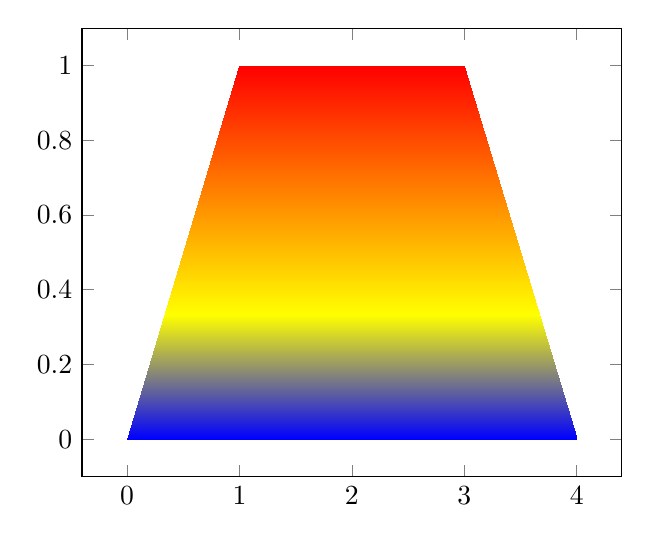
\begin{tikzpicture}
%\tracingmacros=2 \tracingcommands=2
	\begin{axis}
	\addplot[patch,shader=interp]
	table {
		x y z
		0 0 0
		1 1 0
		2 0 0
		%
		1 1 0
		2 0 0
		3 1 0
		%
		2 0 0
		3 1 0
		4 0 0
		%
	};
	\end{axis}
\end{tikzpicture}

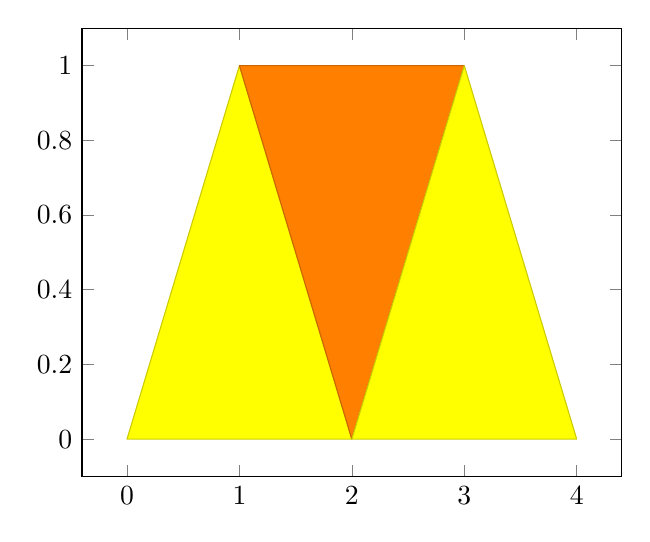
\begin{tikzpicture}
%\tracingmacros=2 \tracingcommands=2
	\begin{axis}
	\addplot[patch]
	table {
		x y z
		0 0 0
		1 1 0
		2 0 0
		%
		1 1 0
		2 0 0
		3 1 0
		%
		2 0 0
		3 1 0
		4 0 0
		%
	};
	\end{axis}
\end{tikzpicture}

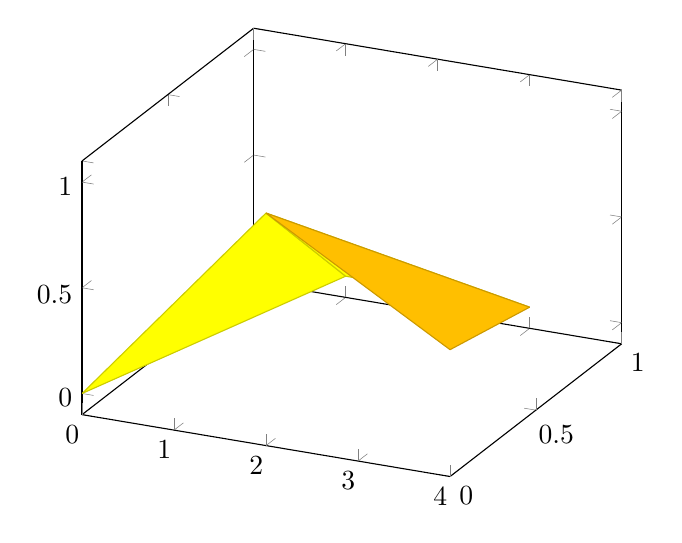
\begin{tikzpicture}
%\tracingmacros=2 \tracingcommands=2
	\begin{axis}
	\addplot3[patch]
	table {
		x y z
		0 0 0
		1 1 0
		2 0 1
		%
		1 1 0
		2 0 1
		3 1 0
		%
		2 0 1
		3 1 0
		4 0 0.5
		%
	};
	\end{axis}
\end{tikzpicture}

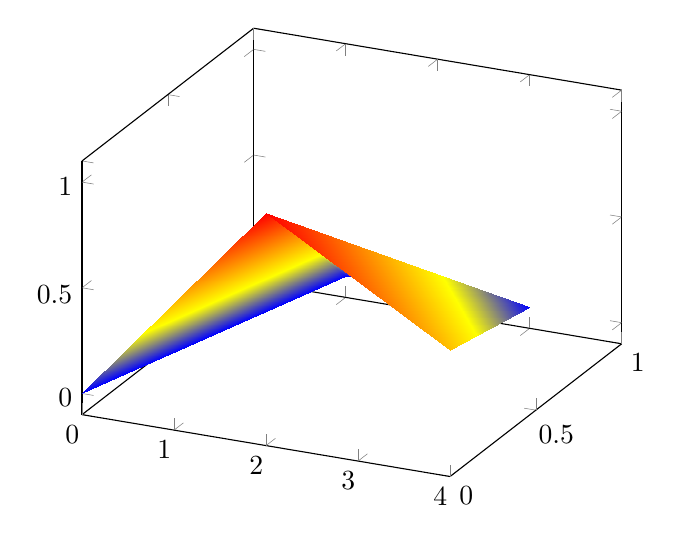
\begin{tikzpicture}
%\tracingmacros=2 \tracingcommands=2
	\begin{axis}
	\addplot3[patch,shader=interp]
	table {
		x y z
		0 0 0
		1 1 0
		2 0 1
		%
		1 1 0
		2 0 1
		3 1 0
		%
		2 0 1
		3 1 0
		4 0 0.5
		%
	};
	\end{axis}
\end{tikzpicture}

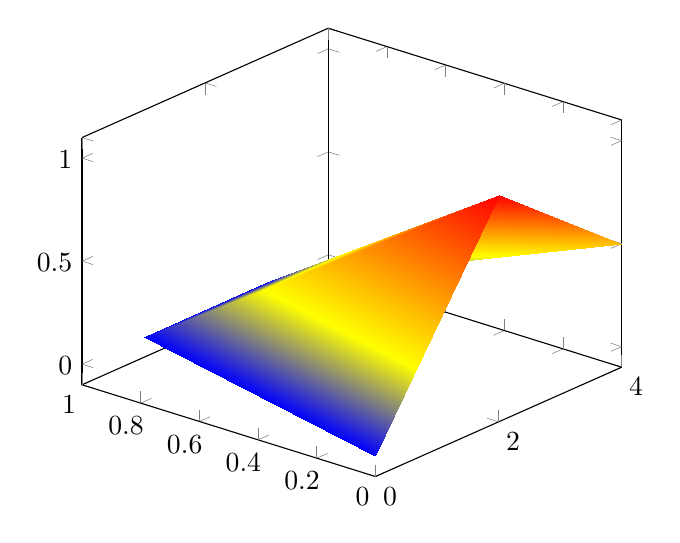
\begin{tikzpicture}
%\tracingmacros=2 \tracingcommands=2
	\begin{axis}[view/h=-50]
	\addplot3[patch,shader=interp]
	table {
		x y z
		0 0 0
		1 1 0
		2 0 1
		%
		1 1 0
		2 0 1
		3 1 0
		%
		2 0 1
		3 1 0
		4 0 0.5
		%
	};
	\end{axis}
\end{tikzpicture}

\input patchplots/patchplottestcolormap.tex

\testsubsection{Solid color}
Matlab:

\message{IF THIS HERE CAUSES AN ERROR, CALL patch_plot_example.m in MATLAB OR OCTAVE}

\matlabtestimg{plot1.png}

PGFPlots:

\begin{tikzpicture}
	\begin{axis}
		\addplot[surf,point meta=\thisrow{c},mesh input=patches] table {patchplots/plot1.dat};
	\end{axis}
\end{tikzpicture}

\testsubsection{Interpolated colors, separate for each patch}
Matlab:

\matlabtestimg{plot2.png}

PGFPlots:

\begin{tikzpicture}
	\begin{axis}
		\addplot[surf,point meta=\thisrow{c},mesh input=patches,shader=interp] table {patchplots/plot2.dat};
	\end{axis}
\end{tikzpicture}

\testsubsection{Interpolated colors, continous over edges}
Matlab:

\matlabtestimg{plot3.png}

PGFPlots:


\begin{tikzpicture}
	\begin{axis}
		\addplot[surf,point meta=\thisrow{c},mesh input=patches,shader=interp] table {patchplots/plot3.dat};
		\addplot[mesh,ultra thin,draw=black,point meta=\thisrow{c},mesh input=patches] table {patchplots/plot3.dat};
	\end{axis}
\end{tikzpicture}

\testsubsection{3D}
Matlab:

\matlabtestimg{plot4.png}

PGFPlots:

\begin{tikzpicture}
	\begin{axis}[view={-37.5}{30}]
		\addplot3[surf,point meta=\thisrow{c},mesh input=patches] table {patchplots/plot4.dat};
	\end{axis}
\end{tikzpicture}

\begin{tikzpicture}
	\begin{axis}[view={-37.5}{30}]
		\addplot3[surf,point meta=\thisrow{c},mesh input=patches,shader=interp] table {patchplots/plot4.dat};
	\end{axis}
\end{tikzpicture}

\testsubsection{3D smooth}
Matlab:

\matlabtestimg{plot5.png}

PGFPlots:

\begin{tikzpicture}
	\begin{axis}[view={-37.5}{30}]
		\addplot3[surf,point meta=\thisrow{c},mesh input=patches] table {patchplots/plot5.dat};
	\end{axis}
\end{tikzpicture}

\begin{tikzpicture}
	\begin{axis}[view={-37.5}{30}]
		\addplot3[surf,point meta=\thisrow{c},mesh input=patches,shader=interp] table {patchplots/plot5.dat};
	\end{axis}
\end{tikzpicture}
